\documentclass[letterpaper]{article}
\synctex=1
\usepackage{graphicx}
\graphicspath{ {images/} }

\usepackage{lipsum}
\usepackage{float}

% \usepackage[
%     style=ieee,
%     backend=biber
%     ]{biblatex}
% \addbibresource{references.bib}

\usepackage{hyperref}

\usepackage{amssymb}

\usepackage{siunitx}

\usepackage{multirow}
% for merging table cells I think

\usepackage{tabularx}
\renewcommand\tabularxcolumn[1]{m{#1}}% for vertical centering text in X column
% allows for linewrap within cells
\newcolumntype{Y}{>{\centering\arraybackslash}X}

\usepackage{todonotes}
\usepackage{pdfpages}

\usepackage{fancyhdr} %header
\fancyhf{}
\renewcommand\headrulewidth{0pt}
\fancyfoot[C]{\thepage}
\renewcommand\footrulewidth{0pt}
\pagestyle{fancy}

\usepackage[pdf]{graphviz}
\usepackage{adjustbox}

\usepackage{amsmath}
\usepackage[smartEllipses]{markdown}

% make subsection use letters
%\renewcommand{\thesubsection}{\alph{subsection}}

%\usepackage{minted}

% \usepackage{amsthm}
\title{ECE 421 Project 2\\
Trees, Trees, and More Trees}
\author{Arun Woosaree\\
Alexander Rostron\\
Jacob Reckhard
}

%actual document
\begin{document}

\maketitle %insert titlepage here

\section{Rationale}
From the beginning, we knew there would be a fair amount of shared functionality
for the Red Black tree and the AVL tree. Therefore, special considerations were
taken to ensure a low level of code duplication, in order to adhere to the DRY
(Don't Repeat Yourself) principle.

\subsection{The Node Trait}\label{dry}
Both the Red Black tree and the AVL tree have nodes, but the Red Black Tree's
nodes need to store colour information, while the AVL tree's nodes need to store
depth information. Thus, a Node trait was created, with default implementations
for getting a string representation of the Node, getting the Node's height, its
size, min, side, sibling, uncle, and determining if the node is a child.

To use this trait, a ColorNode struct, and a DepthNode struct were created,
which have implementations for methods defined by the Node trait but do not have
default implementations. Then, the functionality which is specific to either
ColorNode, or the DepthNode is found in the structs' respective implementation
blocks. This approach allowed us to re-use common functionality between the
different types of nodes, while still allowing for new, separate functionality
defined by the different nodes. 

\subsection{The Tree Trait}
%For the Tree structs for the Red Black tree and AVL trees, we decided to not go
%through the trouble of sharing code. There is a small amount of code
%duplication, but because the tree deals with different types of nodes, we deemed
%it reasonable to have a little bit of code duplication, like the \texttt{find}
%method, for example.
%\todo{are we sharing the trait?}

Both the Red Black tree and the AVL tree share a Tree trait, with
default implementations for insert, delete, rotate, find, get\_height,
and making a string representation of the tree. This prevents us from
having to write and maintain multiple versions of these non trivial
functions. These more complex operations are defined in terms of
simpler operations, and each tree only has to implement these simpler
operations to take advantage of this. Finally, the functionality which is
specific to either the Red Black tree or the AVL tree is implemented
in the Red Black tree struct, and the AVL tree struct, respectively.
(For example, re-balancing the tree after insertion/deletion).  This
approach allowed us to re-use common functionality between the
different types of trees, while still allowing for new, separate
functionality defined by the different trees.

\subsection{Arena based allocation}
The way the memory is allocated for the nodes is a little unusual, in that the
nodes are actually stored in a vector. This allows us to deal with indices,
which reduces the amount of pointers we have to deal with. Essentially, there is
a vector in the tree which contains all the nodes, and each node stores its
parent child relationships as an \texttt{Option<usize>}. This also allowed us to
deal with less headaches dealing with lifetimes and ownership.

\subsection{Unsafe}
In order to return a reference to a value of a vector contained within a
refcell, a raw pointer is used. The unsafe code could be avoided by replacing
each call to self.get(n) with \texttt{\&self.data.borrow()[n]} and each call to
\texttt{self.get\_mut(n)} with \texttt{\&mut self.data.borrow()[n]}. This allows
us to do the same thing with less keystrokes. It does make the program not
thread-safe, but self-balancing trees are a pretty questionable choice for a
multi-threaded data structure anyways, since re-balancing can require that most
of the tree be locked to one thread during an insertion or deletion

\section{Testing}
Several unit tests were created to verify the functionality of the Red Black
tree and the AVL trees.

For both the Red Black tree, and the AVL tree, there are tests to verify:
\begin{enumerate}
  \item the \texttt{contains} function
  \item insertion
  \item printing a string representation of the tree
  \item verifying the tree's height is correct
  \item deletion
\end{enumerate}

Furthermore, tests were created for the \texttt{Node} class. These tests verify
the following functionality:
\begin{enumerate}
  \item getting a children nodes
  \item getting the sibling node
  \item getting uncle nodes
  \item getting the size of a node
  \item getting the height of a node
  \item finding the min value
  \item printing a string representation of the node
\end{enumerate}

\section{Defects}

There are no known faults in the program.
We wrote fairly comprehensive tests, so we feel confident that the trees work as
intended.
%(Or we could mention that the CLI will panic if we haven't handled erroneous
%input yet)

\section{Benchmarking}
Both the Red Black tree and the AVL tree were benchmarked against each other.
Overall, the AVL tree seemed to be faster than the Red Black tree for insertion,
although the benchmark does not test the deletion speed. AVL trees re-balance
more often than Red Black trees, so we would expect deletion to be slower
although this aspect was not benchmarked.  However, it seems like the `manager'
in this case is only concerned with insertion and searching. For small datasets
(about 10000 insertions) the performance difference between the Red Black tree
and the AVL tree seems negligible. However, for this use case we would recommend
the AVL tree, since it is a bit faster, with larger datasets as seen in the
benchmarks below. At 130000 insertions, there is about a 3 ms difference between
the AVL tree and the Red Black tree. This is a big enough difference to prefer
the AVL tree over the Red Black tree for the faster insertions and searching.
If deletion speed was a concern, then the Red Black tree would
likely be a better choice but again, this aspect was not benchmarked since the
focus was on insertion and searching. We used an unbalanced binary search tree
as a baseline, however, the benchmark tests were not feasible to run above the
10000 insertions case for the unbalanced tree since it would take far too long.
Suffice it to say, both the AVL tree and the Red Black trees are many, many
times faster than the unbalanced binary tree for this insertion and search
benchmark.

As such, we decided to include benchmarks for each of the three trees at 10000
insertions, and then comparisons for the Red Black tree and the AVL tree at
130000 insertions. Other benchmarks have been omitted for brevity,
(they would take up way too many pages in this report)
however more benchmarks can be easily run on your machine by running
\verb|cargo bench|, and checking the HTML report generated in the
\texttt{target/} directory.


\begin{figure}[H]
      \centering
      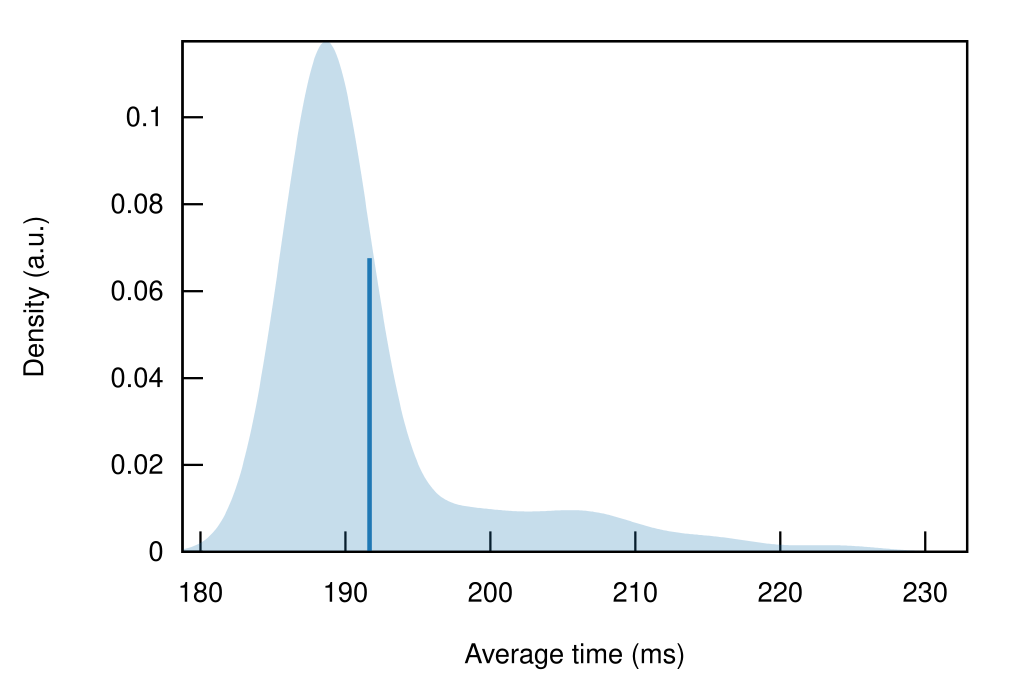
\includegraphics[width=.8\textwidth]{bsbench.png}
      \caption{Unbalanced tree benchmark at 10000 insertions. Out of 100 sample
      taken from 5050 iterations, the mean time to run the benchmark was
    191.67 ms with a median of 188.67 ms}
\end{figure}

\begin{figure}[H]
      \centering
      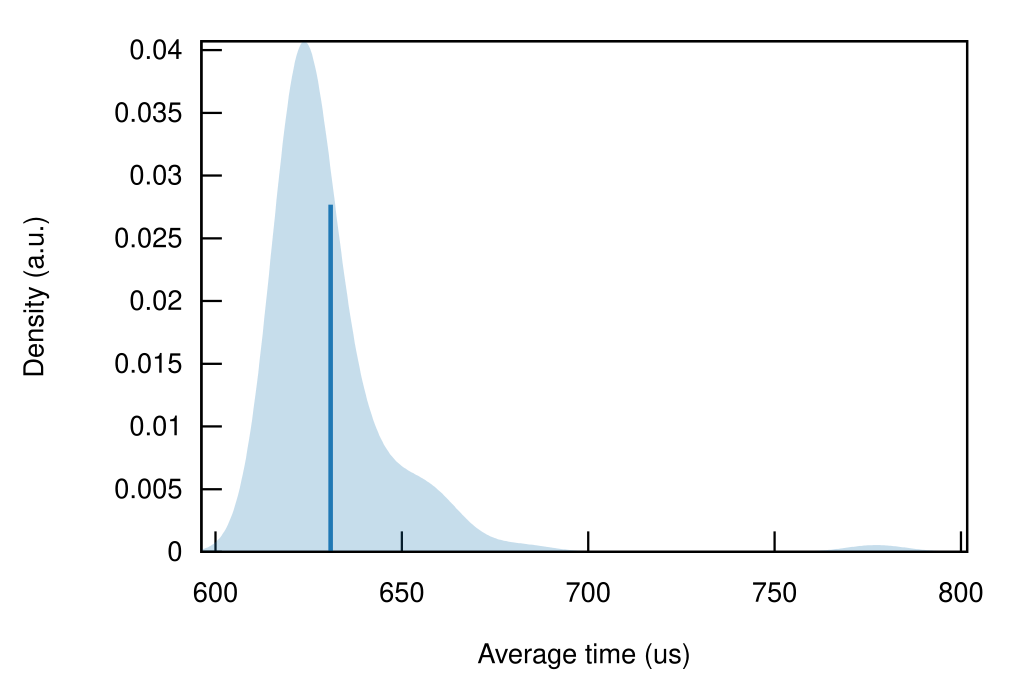
\includegraphics[width=.8\textwidth]{rbsmol.png}
      \caption{Red Black tree benchmark at 10000 insertions. Out of 100 samples
      taken from 5050 iterations, the mean time to run the benchmark was 628.29
    $\mu s$ with a median of 624.55 $\mu s$}
\end{figure}

\begin{figure}[H]
      \centering
      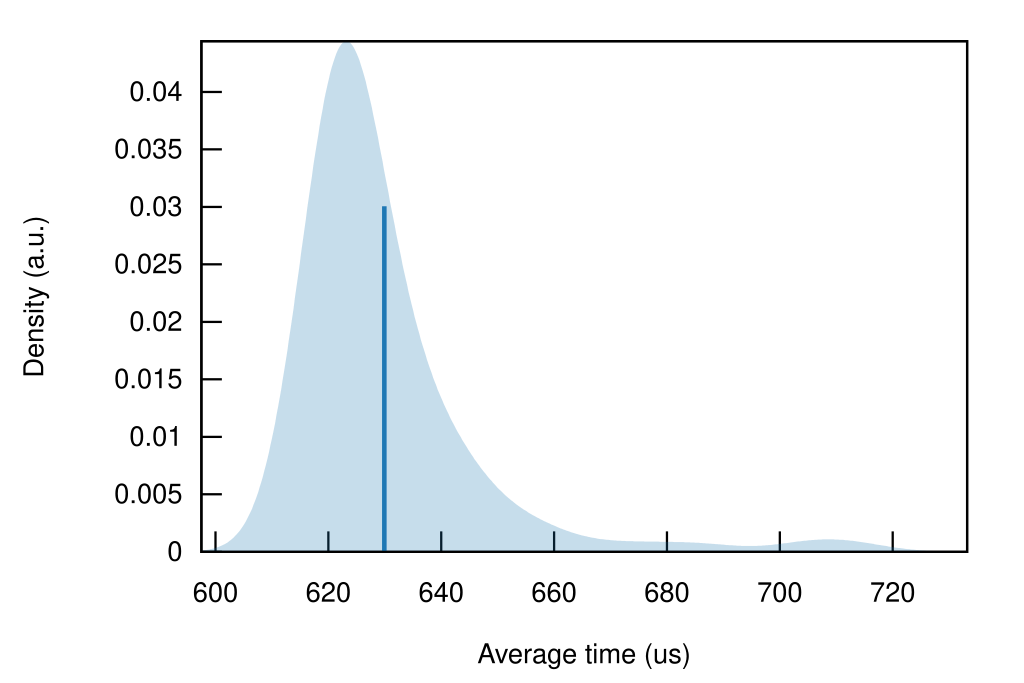
\includegraphics[width=.8\textwidth]{avlsmol.png}
      \caption{AVL tree benchmark at 10000 insertions. Out of 100 samples taken
        from 5050 iterations,
      the mean time to run the benchmark was 627.35 $\mu s$ with a median of
    625.11 $\mu s$}
\end{figure}

\begin{figure}[H]
      \centering
      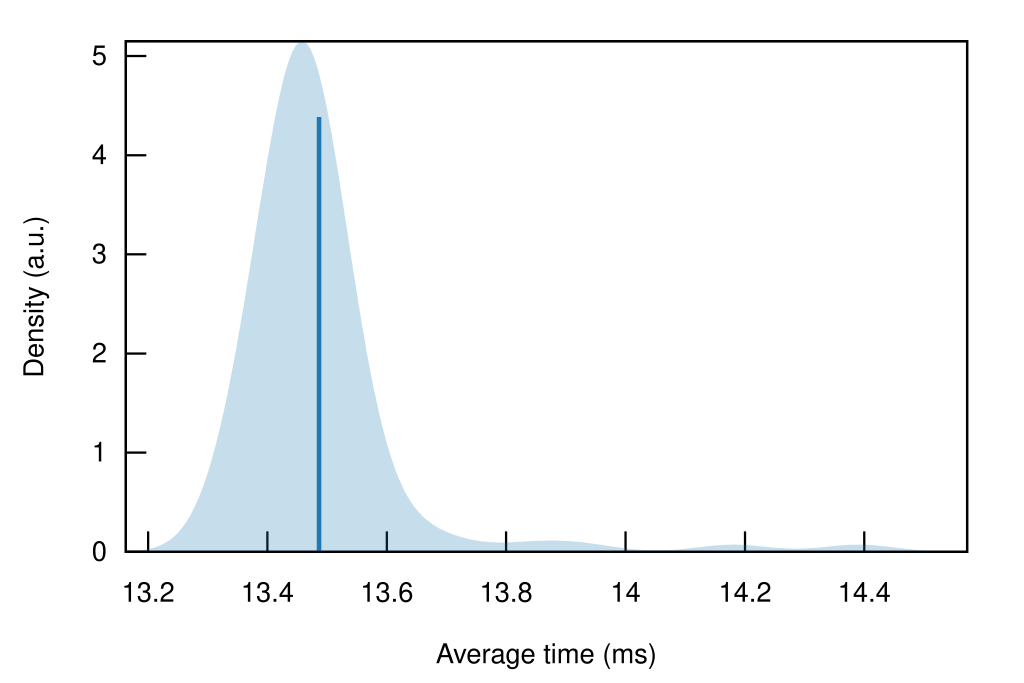
\includegraphics[width=.8\textwidth]{rbbeeg.png}
      \caption{Red Black tree benchmark at 130000 insertions. Out of 100 samples
      taken from 5050 iterations, the mean time to run the benchmark was 13.486
      ms with a median of 13.466 ms}
\end{figure}


\begin{figure}[H]
      \centering
      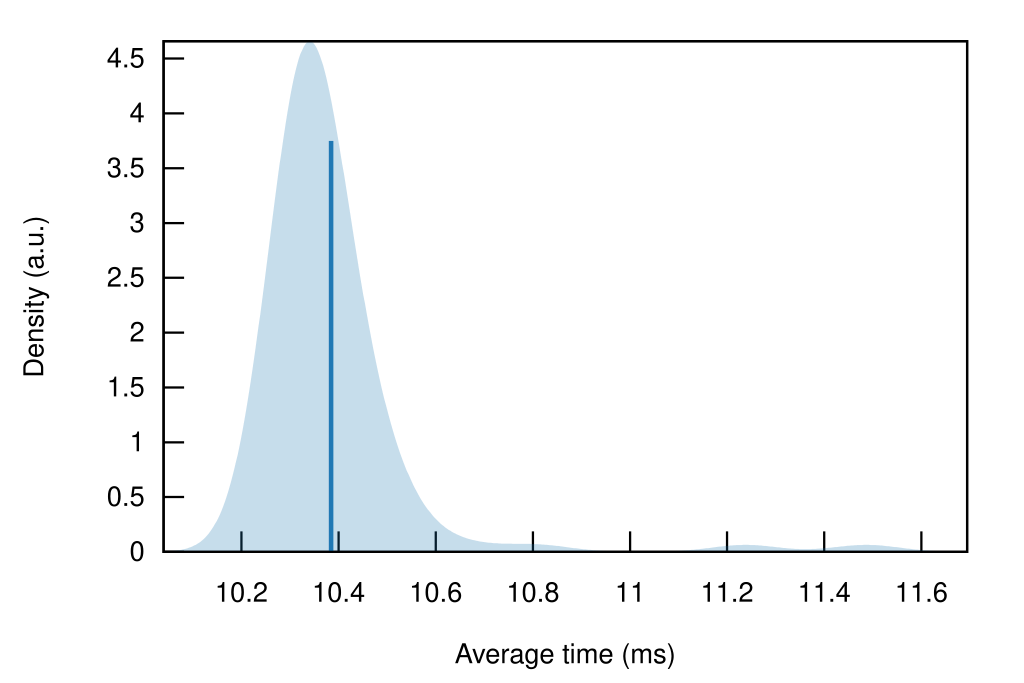
\includegraphics[width=.8\textwidth]{avlbeeg.png}
      \caption{AVL tree benchmark at 130000 insertions. Out of 100 samples
      taken from 5050 iterations, the mean time to run the benchmark was 10.384
    ms with a median of 10.344 ms}
\end{figure}

\section{Additional features}
So-called ``Major innovations''- Additional to the project specification.

\subsection{Helpful macros!}
We decided to create some macros for instantiating the trees.  This will make it
easier for programmers who decide to use our library for some reason to fill
trees with initial values in a nice, convenient, and concise manner.  
Similar to how vectors in Rust have a macro \texttt{vec!}, a Red Black tree,
AVL tree, or unbalanced binary tree can be created using the
following macros:

\begin{texttt}
  redblack!\{1, 2, 3, 4, 5, 6, 7, 8, 9\}
\end{texttt}

\begin{texttt}
  avl!\{1, 2, 3, 4, 5, 6, 7, 8, 9\}
\end{texttt}

\begin{texttt}
  bst!\{1, 2, 3, 4, 5, 6, 7, 8, 9\}
\end{texttt}

\subsection{Pretty tree printing}
We decided to go above and beyond, and have the tree displayed in a pretty
fashion. If the terminal width or height allows for it, a pretty ASCII tree will
be printed. If the user resizes their terminal window, the CLI will also adjust
accordingly.  If there is not enough space to print a pretty tree, the CLI will
fall back to a normal text representation of the tree For Red Black trees, the
colour of the node will also be printed to the terminal! A black node has a
black background colour, while the red nodes have a red background colour.
\begin{figure}[H]
      \centering
      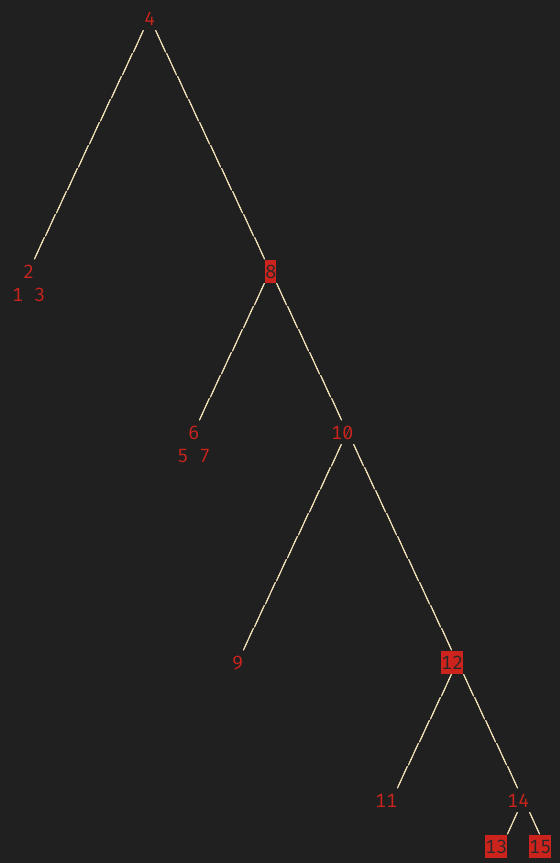
\includegraphics[width=.8\textwidth]{rbtree.png}
      \caption{Pretty visualization for a tree in the CLI.\@ This shows a Red
      Black tree, which also has coloured outputs for the different types of
      nodes}
\end{figure}

For the AVL tree, colouring has be chosen to indicate the balance
factor, with green being a neutral balance factor, yellow being right
heavy, and blue being left heavy.

\begin{figure}[H]
      \centering
      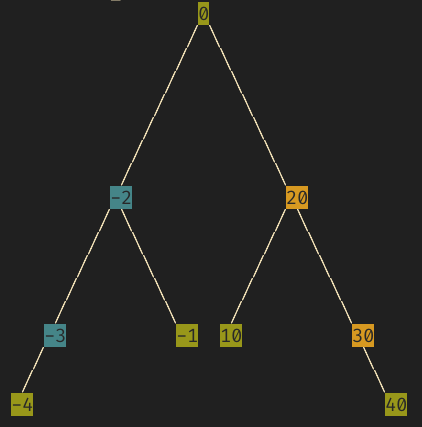
\includegraphics[width=.8\textwidth]{avl.png}
      \caption{Pretty visualization for a tree in the CLI.\@ This shows an AVL
      tree, which also has coloured outputs for the different balance factors}
\end{figure}

%% TODO: insert AVL tree graphic
%% \begin{figure}[H]
%%       \centering
%%       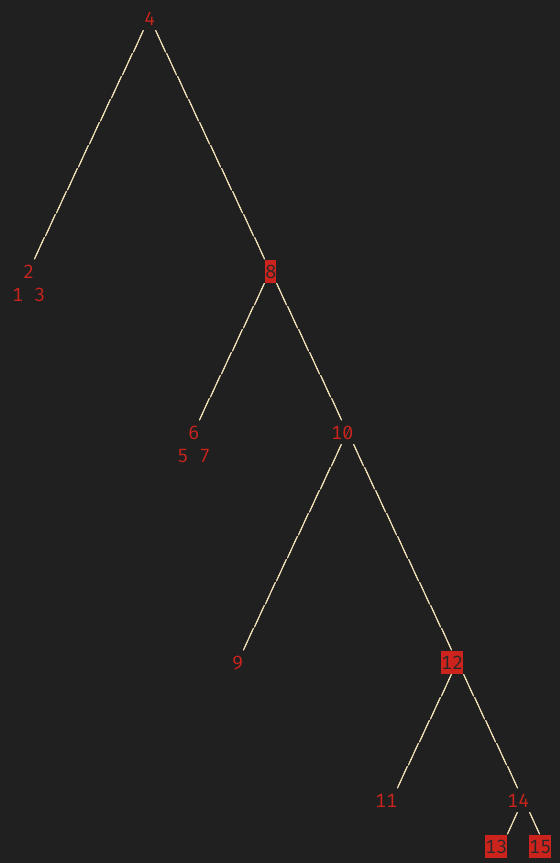
\includegraphics[width=.8\textwidth]{rbtree.png}
%%       \caption{Pretty visualization for a tree in the CLI.\@ This
%%         shows an AVL tree colorized to indicate the balance factor.}
%% \end{figure}

\subsection{Readline buffering}
We also decided to allow the user to easily access previous commands entered in
the CLI simply by pressing the up arrow button. Normally, without this feature,
the following characters would be displayed instead of the previous command that
the user entered, which is not as user-friendly:
\verb|^[[A|


\subsection{Output redirection}
The CLI also supports I/O redirection. If the CLI is invoked and the output is
piped, it will omit unnessesary information, and only output the pretty 

\section{Answers to questions}

\textit{What does a red-black tree provide that cannot be accomplished with
ordinary binary search trees?}

Red Black trees, unlike ordinary Binary Search trees, allow for efficient
in-order traversal (the order Left–Root–Right) of their elements.
Because  height of a Red Black tree remains \(O(\log n)\) after every
insertion and deletion, we can then guarantee that the
upper bound for searching, inserting, deleting, etc is also \(O(\log n)\)
In comparison, an unbalanced Binary Search tree might have a worst-case scenario
of a traversal of size \(O(n)\), for example if every single element was
inserted in ascending or descending order such that each child in the tree is
either all on the left side or all on the right side.

\textit{Please add a command-line interface (function main) to your crate to
allow users to test it.}

Here's a preview of the CLI!
\begin{figure}[H]
      \centering
      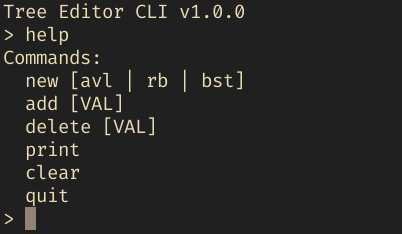
\includegraphics[width=.8\textwidth]{cli.png}
      \caption{A preview of our command-line interface.}
\end{figure}

\textit{Do you need to apply any kind of error handling in your system (e.g.,
panic macro,}
\verb|Option<T>|, \verb|Result<T, E>| \textit{etc..)}

The result and option types are used frequently throughout our
codebase. As part of the parsing for the command line application, the
result type is passed around to account for invalid input. The Option
type is used liberally throughout our tree code, as it's used for
storing both children and parent nodes as there are cases where they
do not exist.

\textit{What components do the Red-black tree and AVL tree have in common? Don’t Repeat
Yourself! Never, ever repeat yourself – a fundamental idea in programming.}

The Red Black tree and the AVL tree have a ColorNode, and a DepthNode,
respectively. These nodes share the Node trait, which we have defined.
Furthermore, the Red Black tree and the AVL tree share a Tree trait, which
handles common functionality such as determining if the tree contains a certain
value.
Please see the design rationale above for more details. \ref{dry}

\textit{How do we construct our design to “allow it to be efficiently and
effectively extended”? For example. Could your code be reused to build a 2-3-4
tree or B tree?}

Actually, with the way we implemented the trees, it would be very easy to re-use
some code to create a 2-3-4 tree, a B tree, or some other type of tree. To
begin, one would have to create a node struct which implements our Node trait,
and then make a tree which implements out Tree trait. From there, the programmer
would simply need to implement the methods without a default implementation.
To make the new tree compatible with out command-line interface, they would need
to add a new tree type to the enum defined in \texttt{main.rs}, and pass it
as an additional argument to the parsing functions in \texttt{main.rs}.


\markdownInput{../README.md}
\end{document}
